\documentclass[tikz, border=10pt]{standalone}
\usepackage{pgfplots}
\pgfplotsset{compat=1.18}

\begin{document}
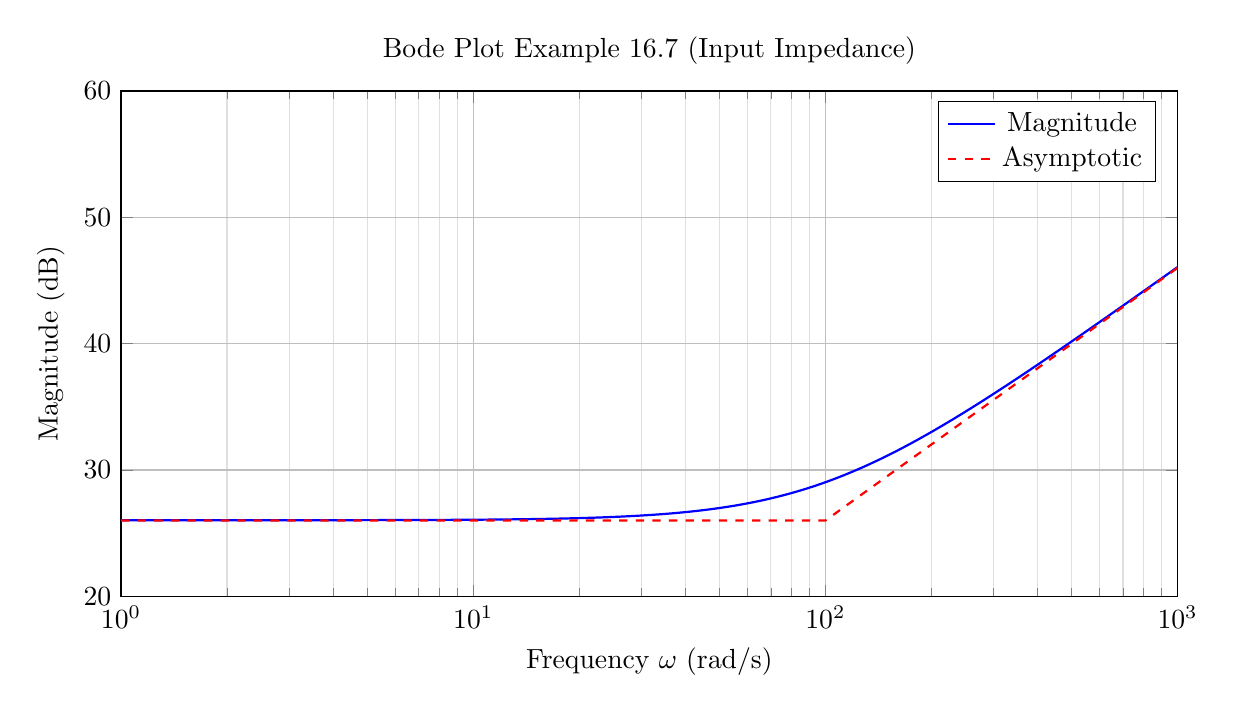
\begin{tikzpicture}
    \begin{semilogxaxis}[
        width=15cm, height=8cm,
        title={Bode Plot Example 16.7 (Input Impedance)},
        xlabel={Frequency $\omega$ (rad/s)},
        ylabel={Magnitude (dB)},
        grid=both,
        xmin=1, xmax=1000,
        ymin=20, ymax=60,
        minor grid style={gray!25},
        major grid style={gray!50},
    ]
    % H(s) = 20(1 + s/100)
    % Magnitude: 20*log10( 20 * sqrt(1 + (x/100)^2) )
    
    \addplot[blue, thick, domain=1:1000, samples=200] {
        20*log10( 20 * sqrt(1 + (x/100)^2) )
    };
    \addlegendentry{Magnitude}
    
    % Asymptotes
    \addplot[red, dashed, thick] coordinates {
        (1, 26) (100, 26) (1000, 46)
    };
    \addlegendentry{Asymptotic}

    \end{semilogxaxis}
\end{tikzpicture}
\end{document}
